% =====================================================================
%  A Knudsen-extended, calendering-aware Zehner-Bauer-Schluender closure
%  for the thermal conductivity of lithium-ion electrode coatings
%
%  Compile (TeXworks): pdfLaTeX, run twice. Bibliography embedded.
%  Figures: vector PDFs in ./figures, regenerated by make_figures.py
%  Code & data: https://github.com/j-stoerk/zehner-electrode-thermal
% =====================================================================
\documentclass[10pt,a4paper]{article}

\usepackage[utf8]{inputenc}
\usepackage[T1]{fontenc}
\input{glyphtounicode}
\pdfgentounicode=1
\usepackage[margin=2.4cm]{geometry}
\usepackage{graphicx}
\usepackage{amsmath,amssymb}
\usepackage{booktabs}
\usepackage{caption}
\usepackage{enumitem}
\usepackage{xcolor}
\usepackage[hidelinks]{hyperref}

\graphicspath{{figures/}}
\captionsetup{font=small,labelfont=bf}
\setlist{itemsep=1pt,topsep=2pt}

\newcommand{\leff}{\lambda_{\mathrm{eff}}}
\newcommand{\lams}{\lambda_{s}}
\newcommand{\lamf}{\lambda_{f}}
\newcommand{\lamg}{\lambda_{g}}
\newcommand{\lamb}{\lambda_{b}}
\newcommand{\Kn}{\mathrm{Kn}}
\newcommand{\WmK}{\,\mathrm{W\,m^{-1}\,K^{-1}}}
\newcommand{\Mzero}{\ensuremath{\mathsf{M0}}}
\newcommand{\Mone}{\ensuremath{\mathsf{M1}}}
\newcommand{\Mtwo}{\ensuremath{\mathsf{M2}}}

\title{\textbf{A Knudsen-extended, calendering-aware Zehner--Bauer--Schl\"under closure for the effective thermal conductivity of lithium-ion electrode coatings and separators}}

\author{Julius St\"ork$^{1,2,\ast}$\\[2pt]
\small $^1$VARTA Microbattery GmbH, Ellwangen, Germany\\
\small $^2$Technische Universit\"at Braunschweig, Braunschweig, Germany\\
\small $^\ast$Corresponding author: \texttt{julius.stoerk@varta-ag.com}\\[2pt]
\small \textit{Draft manuscript, \today}}
\date{}

\begin{document}
\maketitle

% =====================================================================
\begin{abstract}
\noindent
Battery thermal models need the effective through-plane thermal conductivity $\leff$ of every porous layer in the cell, yet the closures supplying it know only the porosity, treat the pore gas as a continuum, and carry no uncertainty statement. We develop and test a Zehner--Bauer--Schl\"under closure that repairs all three gaps. A Smoluchowski/Knudsen correction captures the poor heat conduction of gas in sub-micrometre pores: a systematic $3$--$6\%$ for electrode coatings, and an $84\%$ reduction in polyolefin separators whose pores are narrower than the mean free path of air. A compression-dependent contact term $\varphi(\Pi)$ represents what calendering does: first damaging, then rebuilding the conductive bridges between particles. The closure is differentiable end-to-end, so it runs backwards to turn a thermal measurement into a quality-control reading. Against the open calendering dataset of Gandert et al.\ (four electrode types, 27 states), the zero-parameter model predicts the assumption-matching electrode (uncalendered NMC811) to $+2.7\%$ and beats the classical effective-medium baselines. Adding the contact physics lowers the mean error from $31.1\%$ to $4.5\%$ -- the measurement noise floor -- and reproduces, for the first time to our knowledge, the experimentally observed u-shaped conductivity--calendering dependence; Bayesian inference and information criteria confirm both the calibration and the necessity of the term. A bottom-up prediction of a measured 18650 cell lands within $+15\%$. Calibration transfer between recipes is governed by one physically meaningful parameter, yielding design rules, and the inverse mode recovers coating porosity to $\pm0.008$ from one noisy measurement. A falsifiable two-gas-pressure campaign is specified.
\end{abstract}

\vspace{1ex}
\noindent\textbf{Keywords:} effective thermal conductivity; lithium-ion battery; calendering; Knudsen effect; effective-medium theory; inline quality control

% =====================================================================
\section{Introduction}
\label{sec:intro}

Thermal management decides how long a lithium-ion battery lives and how safely it operates. Elevated temperatures accelerate the side reactions that consume capacity, temperature \emph{gradients} across a cell make its regions age at different rates, and in the worst case a local hot spot can trigger thermal runaway \cite{bandhauer2011,richter2017}. Designing against all three requires thermal \emph{models}, and every such model needs the effective through-plane thermal conductivity $\leff$ of each layer in the stack as an input. Through-plane conduction is the bottleneck: cell-level cross-plane values of $0.15$--$0.8\WmK$ lie roughly two orders of magnitude below the in-plane values \cite{richter2017,steinhardt2022}, so heat generated in the interior must cross many poorly conducting porous layers before it can leave the cell.

Moreover, $\leff$ depends strongly on processing. Calendering, the roll-pressing step that compacts a coated electrode to its target porosity, changes the conductivity substantially: in the measurements of Gandert et al.\ \cite{gandert2023}, calendering a graphite anode from porosity $\varepsilon=0.60$ down to $\varepsilon=0.21$ raised the measured electrode conductivity from about $1.5$ to $2.4\WmK$, a change of roughly $60\%$. A thermal model that treats $\leff$ as a handbook constant therefore embeds a hidden, process-dependent error which, once wetting state and porosity are both accounted for, approaches an order of magnitude.

Decades of research on heat conduction in packed beds and porous media have produced closures, compact formulas that predict $\leff$ from the constituent conductivities and the pore structure, and the Zehner--Bauer--Schl\"under (ZBS) family \cite{zehner1970,bauer1978,vdi} is the most widely used of them, including for battery components \cite{oehler2021,gandert2023}. Yet recent measurements expose a structural mismatch between what these closures describe and what electrode manufacturing produces. Three gaps stand out.

\emph{(i) The pore gas is not a continuum.} Electrode pores measure a few micrometers and separator pores only tens of nanometers, while an air molecule travels on average $67$\,nm between collisions at ambient conditions \cite{kennard1938}. In such pores, gas conducts heat far worse than the handbook value suggests (Sec.~\ref{sec:model:knudsen} quantifies this). The effect is well known in insulation research, but it has not been built into ZBS-based battery modelling; Gandert et al.\ \cite{gandert2023} explicitly flag it as a known but unquantified correction in their own data evaluation.

\emph{(ii) Porosity alone cannot describe calendering.} Gandert et al.\ measured four electrode types across 27 calendering states and found a \emph{non-monotonic, u-shaped} dependence of $\leff$ on porosity, which correlates with the adhesion between coating and current collector. They compared two state-of-the-art models, an analytic homogenization closure \cite{oehler2021} and a discrete-element simulation \cite{sangros2017}, and reported poor agreement: both rise monotonically as porosity falls, because both see only the pore volume, while calendering acts on the \emph{contacts} between particles.

\emph{(iii) Closures are only ever run forwards.} Their potential as \emph{inverse} tools, reading porosity or interface quality back from a fast thermal measurement, is unexploited, although interface quality dominates the thermal resistance of a cell stack \cite{vishwakarma2015} and currently has no inline monitor at all.

This paper closes these gaps with a deliberately minimal extension of the ZBS closure, validated and calibrated on openly published data. Our contributions are:

\begin{itemize}
\item[\textbf{C1}] \textbf{A Knudsen-extended ZBS closure} for battery components (Sec.~\ref{sec:model:knudsen}). We quantify a correction that has previously been noted but not evaluated for battery components: 3\% to 6\% for electrodes under laser-flash conditions (helium atmosphere), and $-84\%$ of pore-gas conduction for polyolefin separators, where we additionally show that classical continuum sphere-pack models match measurements only through a cancellation of two errors (Sec.~\ref{sec:results:baselines}).
\item[\textbf{C2}] \textbf{A calendering-aware contact term} $\varphi(\Pi)$ (Sec.~\ref{sec:model:contact}), to our knowledge the first closure that reproduces the measured u-shape. An ablation (Sec.~\ref{sec:results:ablation}) attributes the error reduction, $31.1\%\to13.5\%\to4.5\%$, to its individual components; the endpoint is the dataset's own noise floor.
\item[\textbf{C3}] \textbf{An error, identifiability, and transfer analysis} (Sec.~\ref{sec:results:errors}). A profile-likelihood study bounds which parameters the data can and cannot determine; hybrid-swap experiments show that cross-recipe transfer failure is carried by one parameter, the as-coated bridge conductance, giving a one-measurement re-anchoring rule and volume-space design principles for additive and binder selection (Sec.~\ref{sec:results:design}); Bayesian posteriors and WAIC information criteria corroborate both the calibration and the necessity of the process-dependent contact term (Sec.~\ref{sec:results:bayes}).
\item[\textbf{C4}] \textbf{Differentiable inverse tools for manufacturing quality control} (Sec.~\ref{sec:results:qc}): coating porosity from a single $3\%$-noise thermal reading to $\pm0.008$ absolute with a calibrated uncertainty, and a bridge/core decomposition that makes thermal metrology the first candidate inline monitor for interface and delamination quality.
\item[\textbf{C5}] \textbf{A falsifiable experimental program} (Sec.~\ref{sec:experiments}), centered on a two-gas-pressure protocol that separates pressure-dependent pore-gas conduction from pressure-independent skeleton conduction, testing the mechanism rather than the fit.
\end{itemize}

All code, data transcriptions, and analysis notebooks are openly available at \url{https://github.com/j-stoerk/zehner-electrode-thermal} (Reproducibility Statement).

% =====================================================================
\section{Related work}
\label{sec:related}

\paragraph{Analytic effective-medium closures.}
The classical results bracket what any two-phase mixture can conduct: the Wiener bounds \cite{wiener1912} are the exact best and worst cases (all material in parallel, or all in series), tightened by the Hashin--Shtrikman bounds \cite{hashin1962} for isotropic mixtures. Structure-specific models then commit to a particular geometry. Maxwell--Eucken \cite{maxwell1891,eucken1932} pictures isolated particles floating in a connected fluid; Bruggeman's effective-medium theory \cite{bruggeman1935} treats both phases as interpenetrating; the ZBS family \cite{zehner1970,bauer1978,vdi} resolves a packed-bed unit cell in which particles touch at points (or, in Bauer's extension, over small flattened contacts). All of these evaluate in microseconds, differentiate cleanly, and have parameters one can reason about, which is why they dominate engineering practice. Their weakness is the flip side of their strength: each is only as good as its geometric commitment. We turn this weakness into a diagnostic in Sec.~\ref{sec:results:baselines}, where the \emph{pattern} of baseline failures (Bruggeman matching co-continuous separators but overshooting sphere-packed electrodes by up to $+465\%$, Maxwell--Eucken undershooting everywhere) identifies the governing microstructure of each component. None of these closures, as used for batteries, includes rarefied-gas corrections or any process variable beyond porosity.

\paragraph{Microstructure-resolved simulation.}
Discrete-element models \cite{sangros2017} and homogenization on real or virtual microstructures \cite{oehler2021} represent particle arrangements explicitly, and can in principle resolve contact areas. In practice, both approaches were reduced to porosity-parameterized predictions when compared against the calendering data, and both missed the u-shape \cite{gandert2023}: their structure generators do not encode how a calender damages and rebuilds contacts. Resolved simulation also costs orders of magnitude more per evaluation than a closure and does not differentiate conveniently, which forecloses the inverse applications of Sec.~\ref{sec:results:qc}. Our approach is complementary rather than competitive: keep closure-level cost and differentiability, and inject the missing contact physics through a low-dimensional, process-indexed term whose parameters are interpretable and cheap to calibrate (about six calendering states).

\paragraph{Rarefied gas conduction in confined pores.}
That gas conducts poorly in pores comparable to its molecular mean free path is textbook kinetic theory \cite{kennard1938} and is quantitatively central to insulation and aerogel engineering \cite{kaganer1969}, where pore sizes resemble those of battery separators. Coupling this effect into the ZBS framework for battery components appears to be missing from the literature, and the authors of the primary dataset name it as an open issue \cite{gandert2023}. Sec.~\ref{sec:model:knudsen} supplies the term, and Sec.~\ref{sec:experiments} the experiment that isolates it: gas conduction depends on pressure, skeleton conduction does not.

\paragraph{Battery component thermal measurements.}
Component-level data come from steady-state stacked-sample rigs with controlled compaction \cite{burheim2013,richter2017}, copper-block reference-bar setups on cell teardowns \cite{marconnet2018,vishwakarma2015}, and flash-diffusivity metrology with penetration-model evaluation \cite{mcmasters,gandert2023}; canonical early values are due to Maleki et al.\ \cite{maleki1999}. Two robust experimental findings frame our work: soaking a coating with electrolyte raises its conductivity roughly threefold \cite{burheim2013,marconnet2018}, and interfaces, not bulk layers, dominate stack resistance \cite{vishwakarma2015}. The first is a clean test of any closure's fluid sensitivity; the second both motivates our contact term and warns that stack-derived literature values are lower bounds for single coatings.

% =====================================================================
\section{Model}
\label{sec:model}

\subsection{Setting, notation, and assumptions}
\label{sec:model:setup}

We model a porous coating as a two-phase medium: solid particles of conductivity $\lams$ and diameter $d_p$, and a pore fluid of conductivity $\lamf$ (a gas or the liquid electrolyte), at porosity $\varepsilon$ (the pore volume fraction). The closure predicts the dimensionless ratio $k_{\mathrm{bed}}=\leff/\lamf$ as a function of $\varepsilon$ and the phase contrast $\kappa=\lams/\lamf$. Calendering is indexed by the compression rate
\begin{equation}
\Pi \;=\; 1-\frac{s_{\mathrm{co}}}{s_{\mathrm{co},0}},
\label{eq:Pi}
\end{equation}
where $s_{\mathrm{co}}$ is the coating thickness after calendering and $s_{\mathrm{co},0}$ the as-coated thickness, so $\Pi=0$ means uncalendered and $\Pi=0.5$ means compressed to half thickness. Our assumptions, stated up front:

\begin{itemize}
\item[\textbf{A1}] Steady diffusive heat conduction only. Radiation and convection inside the pores are negligible at micrometer pore sizes and ambient temperature (we verified the porous-convection threshold is missed by about fifteen orders of magnitude at coating scale).
\item[\textbf{A2}] The closure's unit cell assumes a statistically isotropic packing of spheres. Real deviations are not re-meshed but absorbed into interpretable parameters: the strong conductivity anisotropy of graphite flakes goes into an effective $\lams$ that must stay inside the single-crystal anisotropy band, and all solid--solid contact conduction goes into the contact term of Sec.~\ref{sec:model:contact}.
\item[\textbf{A3}] The pore gas behaves as a continuum except for the conductivity reduction of Eq.~\eqref{eq:knudsen}; the liquid electrolyte needs no such correction because molecular mean free paths in liquids are sub-nanometer.
\item[\textbf{A4}] A single scalar $\varphi$ stands for the area fraction of all conductive solid--solid bridges (particle--particle necks, binder/carbon-black bridges, coating--collector contact), and the bridge material may differ from the particles, with its own conductivity $\lamb$.
\item[\textbf{A5}] Within one electrode family (one recipe and coating process), the material parameters $(\lams,\lamb,\varphi_0,a,b)$ are constants; only $\varepsilon$ and $\Pi$ change along the calendering trajectory.
\end{itemize}

Why build on ZBS rather than on one of the other closures of Sec.~\ref{sec:related}? Three reasons guided the choice. First, \emph{morphology}: electrodes really are packings of particles, so ZBS's unit cell is the right starting picture, whereas Maxwell--Eucken's isolated particles and Bruggeman's interpenetrating phases are not (Sec.~\ref{sec:results:baselines} confirms this empirically). Second, \emph{validation headroom}: the base closure was validated in companion work on Zehner's original packed-bed data across phase contrasts $\kappa\in[4,\,14094]$, and the battery systems' values ($\kappa=14$--$1005$) lie strictly inside that range, so we \emph{interpolate} in $\kappa$ and extrapolate only in porosity (examined empirically in Sec.~\ref{sec:results:errors}). Third, \emph{extensibility}: ZBS fails on battery components at exactly two nameable points, the pore-gas conductivity and the contact term, and both can be repaired without touching the rest of the model.

\subsection{Base closure (\Mzero)}
\label{sec:model:zbs}

The ZBS closure \cite{zehner1970,bauer1978,vdi} pictures the bed as two parallel channels: a pure-fluid channel of relative cross-section $1-\sqrt{1-\varepsilon}$, and a particle-core channel of cross-section $\sqrt{1-\varepsilon}$ in which heat must pass through fluid gaps between curved particle surfaces:
\begin{equation}
k_{\mathrm{bed}}(\varepsilon,\kappa) \;=\; \underbrace{1-\sqrt{1-\varepsilon}}_{\text{fluid channel}} \;+\; \underbrace{\sqrt{1-\varepsilon}\;\lambda_{pm}(\varepsilon,\kappa)}_{\text{particle-core channel}} .
\label{eq:zbs}
\end{equation}
The core term $\lambda_{pm}$ results from integrating the local series resistance across the unit cell:
\begin{equation}
\lambda_{pm}=\frac{2}{1-B/\kappa}\!\left[\frac{B(\kappa-1)}{\kappa\,(1-B/\kappa)^{2}}\,\ln\frac{\kappa}{B}\;-\;\frac{B+1}{2}\;-\;\frac{B-1}{1-B/\kappa}\right],
\qquad
B = C\left(\frac{1-\varepsilon}{\varepsilon}\right)^{10/9},
\label{eq:lampm}
\end{equation}
where $B$ is the particle deformation parameter (it controls how strongly the unit-cell particle is flattened) and $C$ a shape factor, $C=1.25$ for spheres. The structure of Eq.~\eqref{eq:zbs} is worth a moment of reflection, because it explains the model's behavior later. In the limit $\varepsilon\to1$ the fluid channel takes over and $k_{\mathrm{bed}}\to1$, as it must. For large phase contrast $\kappa$, the core term grows only logarithmically, because the bottleneck is the thin fluid gap where the particles approach each other: no matter how conductive the particles are, heat must squeeze through that gap. This is precisely why the model \emph{under}-predicts whenever real coatings provide solid bridges across the gap, and why a contact term is the physically correct repair rather than, say, inflating $\lams$. Equations~\eqref{eq:zbs}--\eqref{eq:lampm} with continuum $\lamf$ constitute our baseline \Mzero{}.

\subsection{Knudsen-corrected pore gas}
\label{sec:model:knudsen}

Gas conducts heat by molecules colliding and passing kinetic energy along. When the pore becomes comparable to the mean free path, the average distance a molecule travels between collisions, a molecule crosses the pore and hits the wall before it ever meets another molecule: the pore gas stops behaving like a heat-carrying medium and becomes a lonely messenger bouncing down an empty corridor. The standard correction (often attributed to Smoluchowski) writes the effective gas conductivity as
\begin{equation}
\lambda_{g,\mathrm{eff}}
=\frac{\lamg}{1+2\beta\,\Kn},
\qquad
\Kn=\frac{\Lambda}{d_{\mathrm{pore}}},
\qquad
\Lambda=\frac{k_{B}T}{\sqrt{2}\,\pi d_{g}^{2}\,p},
\label{eq:knudsen}
\end{equation}
where $\lamg$ is the continuum gas conductivity, $\Kn$ the Knudsen number, $\Lambda$ the mean free path, $d_{\mathrm{pore}}$ the pore diameter, $k_B$ the Boltzmann constant, $T$ the absolute temperature, $p$ the gas pressure, $d_g$ the effective molecular collision diameter (so $\Lambda_{\mathrm{air}}\approx67$\,nm and $\Lambda_{\mathrm{He}}\approx190$\,nm at ambient conditions), and $\beta$ a dimensionless jump coefficient of order unity that bundles the gas--surface energy accommodation; we use $\beta=1.64$, a standard value for air on technical surfaces, and quantify the sensitivity to this choice in Sec.~\ref{sec:results:errors}. Two limits anchor the formula: for $\Kn\to0$ (large pores) the continuum value is recovered, which is why packed beds of millimeter particles never needed this correction; for $\Kn\to\infty$ the gas conduction vanishes entirely. The pore size follows the hydraulic estimate for sphere packings,
\begin{equation}
d_{\mathrm{pore}}=\frac{2}{3}\,\frac{\varepsilon}{1-\varepsilon}\,d_{p},
\label{eq:dpore}
\end{equation}
or is taken from porosimetry where available (polyolefin separators: $43$--$64$\,nm). The corrected contrast $\kappa_{\mathrm{eff}}=\lams/\lambda_{g,\mathrm{eff}}$ then enters Eq.~\eqref{eq:zbs} unchanged. Note the practical subtlety this introduces: the ``dry'' conductivity of a coating now depends on \emph{which gas} fills the pores and at \emph{what pressure}, so a laser-flash measurement under helium purge probes a different pore-gas state than a coating sitting in air, and both differ from a coating under vacuum. Section~\ref{sec:experiments} exploits this pressure dependence as a validation experiment.

\subsection{Calendering-aware contact term}
\label{sec:model:contact}

Calendering acts on contact zones, not on pore volume, which is the root reason porosity-only models cannot represent its signature. To give the closure eyes for contacts, we adopt the flattened-contact generalization of Eq.~\eqref{eq:zbs} from the VDI Heat Atlas \cite{vdi} and extend it with a bridge phase whose conductivity may differ from the particles':
\begin{equation}
k_{\mathrm{bed}}
= 1-\sqrt{1-\varepsilon}+\sqrt{1-\varepsilon}\,
\Bigl[\varphi\,\frac{\lamb}{\lamf} + (1-\varphi)\,\lambda_{pm}(\varepsilon,\kappa)\Bigr],
\label{eq:contact}
\end{equation}
where $\varphi$ is the fraction of the particle-channel cross-section occupied by solid bridges and $\lamb$ is the conductivity of whatever forms those bridges: graphite--graphite flake contacts ($\lamb\approx130\WmK$) in anodes, the carbon-black/binder network ($\lamb\approx24\WmK$, the carbon-black value cited in \cite{gandert2023}) between NMC particles in cathodes. The product $\varphi\,\lamb$ is the physically meaningful group, an areal bridge conductance: doubling the bridge area at half the bridge conductivity leaves the heat flow unchanged, and Sec.~\ref{sec:results:errors} shows the data indeed determine this product more robustly than its factors. Setting $\varphi=0$ recovers \Mzero{} exactly, a property we enforce in the code by regression test.

How should $\varphi$ depend on calendering? The dataset's own adhesion measurements give the answer: Gandert et al.\ \cite{gandert2023} observe that coating--collector adhesion first \emph{drops} with calendering (the roll gap shears the coating and damages the as-coated binder network) and then \emph{recovers} at high line loads (particles interlock and even press into the soft aluminum foil, which they document by electron microscopy). Calendering, in short, first burns the bridges it later rebuilds. The lowest-order polynomial able to express a dip followed by a recovery is a quadratic, so we set
\begin{equation}
\varphi(\Pi)=\max\!\bigl(0,\;\varphi_{0}+a\,\Pi+b\,\Pi^{2}\bigr),
\label{eq:phi}
\end{equation}
with three nameable coefficients: $\varphi_0>0$ is the as-coated bridge fraction (expected near the rigid-sphere contact value of $0.0077$ tabulated in the VDI Heat Atlas), $a<0$ is the shear-damage rate, and $b\ge0$ is the interlocking recovery, a threshold effect that a gentle process window may simply never reach. We considered and rejected richer forms: a piecewise-linear $\varphi(\Pi)$ adds a breakpoint parameter that the six to eight data points per family cannot support, and an exponential decay-plus-growth form fits no better while hiding the dip location inside a nonlinear combination of rates. The quadratic is the most parsimonious shape that can be falsified by the adhesion correlation proposed in Sec.~\ref{sec:experiments}. We write \Mone{} for Eqs.~\eqref{eq:contact}--\eqref{eq:phi} restricted to constant $\varphi$ ($a=b=0$) and \Mtwo{} for the full quadratic.

\subsection{Differentiable implementation and inverse use}
\label{sec:model:inverse}

Equations~\eqref{eq:zbs}--\eqref{eq:phi} are implemented in JAX with 64-bit precision, which means every derivative of the model is available exactly, by automatic differentiation, rather than by finite differences with their step-size headaches. The inverse map for porosity quality control is Newton's iteration
\begin{equation}
\varepsilon_{k+1}=\varepsilon_{k}-\frac{\leff(\varepsilon_{k})-\lambda^{\mathrm{meas}}}{\partial\leff/\partial\varepsilon\,(\varepsilon_{k})},
\label{eq:newton}
\end{equation}
where $\lambda^{\mathrm{meas}}$ is the measured conductivity and $\varepsilon_k$ the porosity estimate at iteration $k$; the iteration converges quadratically because the derivative is exact, and the solution is unique because $\leff(\varepsilon)$ is strictly monotonic over the relevant porosity range (verified numerically; intuitively, more pores always means less conduction once the contact state is fixed). First-order uncertainty propagation turns measurement and model noise into a porosity error bar:
\begin{equation}
\sigma_{\varepsilon}
=\frac{\sqrt{\sigma_{\mathrm{meas}}^{2}+\sigma_{\mathrm{model}}^{2}}\;\leff}
{\bigl|\partial\leff/\partial\varepsilon\bigr|},
\label{eq:sigma}
\end{equation}
where $\sigma_{\mathrm{meas}}$ is the relative noise of the conductivity measurement (laser flash or transient plane source: typically $2$--$5\%$) and $\sigma_{\mathrm{model}}$ a relative model-form floor, which we set to $2\%$, the residual scatter of the base closure's packed-bed validation. The formula also explains \emph{which} electrode makes the best QC target: the larger the sensitivity $|\partial\leff/\partial\varepsilon|$, the smaller the porosity uncertainty, and the anode has the largest sensitivity of the three components.

% =====================================================================
\section{Data, baselines, and calibration protocol}
\label{sec:data}

\subsection{Primary dataset}
\label{sec:data:primary}
Gandert et al.\ \cite{gandert2023} (open access, CC-BY) measured two graphite anodes on copper foil (96\,wt\% active material, CMC/SBR binder, 1.5\% carbon black; two coating thicknesses) and NMC622/NMC811 cathodes on aluminum foil (PVDF binder; NMC622 additionally 2\,wt\% flake-graphite additive), each calendered on a laboratory roll calender to six to eight states. Conductivity follows from $\lambda=\kappa_d\,\rho\,c_p$, where $\kappa_d$ is the laser-flash thermal diffusivity (measured under \emph{helium} purge with penetration-model evaluation \cite{mcmasters}), $c_p$ the specific heat from differential scanning calorimetry, and $\rho$ the density from gas pycnometry; thicknesses come from a flat-anvil micrometer at contact pressures below $0.3\,\mathrm{N\,mm^{-2}}$ (the authors show that ball-tip dial gauges compress the coating and read up to $23\%$ low); porosity uncertainties follow the Guide to the Expression of Uncertainty in Measurement. We transcribe their per-sheet porosities and thicknesses and evaluate their published fit functions at those porosities. The metal foil is removed by series subtraction,
\begin{equation}
\frac{s_{\mathrm{co}}}{\lambda_{\mathrm{co}}}
=\frac{s_{\mathrm{stack}}}{\lambda_{\mathrm{stack}}}-\frac{s_{\mathrm{cc}}}{\lambda_{\mathrm{cc}}},
\label{eq:stack}
\end{equation}
where subscripts co, stack, and cc denote coating, coated stack, and current collector, $s$ are thicknesses and $\lambda$ conductivities ($\lambda_{\mathrm{Cu}}=400$, $\lambda_{\mathrm{Al}}=237\WmK$; the foil term is below $0.1\%$ of the total). One systematic remains by construction: the coating/collector contact resistance stays lumped inside $\lambda_{\mathrm{co}}$, exactly as in the source. Because the flash measurements run under helium, all dry comparisons use helium as the pore gas ($\lamg=0.1518\WmK$), and since $\Lambda_{\mathrm{He}}\approx190$\,nm is almost three times the air value, this dataset stresses the Knudsen term roughly three times harder than air would: an accident of metrology that works in the validation's favor.

\subsection{Anchor datasets}
Independent anchors, compiled with row-level citations in the repository: dry polyolefin separators $0.07$--$0.18\WmK$ across types and compaction pressures \cite{richter2017}; a ceramic-coated separator stack at $0.10$ dry and $0.11$ wet \cite{marconnet2018}; soaked/dry electrode pairs, graphite $0.30\to0.89$ and LCO $0.36\to1.10\WmK$ \cite{burheim2013}, CMS graphite $0.57\to1.35$ and LMO $0.16\to0.45\WmK$ \cite{marconnet2018}; the interface-dominance result of \cite{vishwakarma2015}; separator pore sizes ($43$--$64$\,nm) from porosimetry. Constituent properties used throughout: $\lambda_{\mathrm{air}}=0.026$, $\lambda_{\mathrm{electrolyte}}=0.18\WmK$ (carbonate-solvent class \cite{maleki1999}), particle sizes $d_p=18\,\mu$m (graphite) and $10\,\mu$m (NMC). For the cell-level test of Sec.~\ref{sec:results:stack} we additionally use the complete layer structure (thicknesses and porosities per layer) and the measured jelly-roll conductivity of a commercial 18650 cell, $k_\perp = 1.122\WmK \pm 6.2\%$ \cite{steinhardt2021}, the meta-analytic range of all published cell-level values, $0.15$--$1.4\WmK$ \cite{steinhardt2022}, and, as a cross-model anchor, microstructure-resolved simulation results for electrolyte-filled coatings \cite{oehlerdiss}.

\subsection{Baselines}
\label{sec:data:baselines}
We compare against the classical closure hierarchy, all evaluated with the \emph{same} constituent properties and the same Knudsen-corrected pore gas, so that differences isolate the geometric assumptions rather than the inputs. The Wiener bounds \cite{wiener1912} are the parallel and series arrangements. Maxwell--Eucken \cite{maxwell1891,eucken1932}, for isolated solid spheres of volume fraction $1-\varepsilon$ dispersed in connected fluid, reads
\begin{equation}
\leff^{\mathrm{ME}}
=\lamf\,\frac{\lams+2\lamf+2(1-\varepsilon)(\lams-\lamf)}{\lams+2\lamf-(1-\varepsilon)(\lams-\lamf)},
\label{eq:me}
\end{equation}
and Bruggeman's symmetric effective-medium theory \cite{bruggeman1935}, which treats both phases as interpenetrating, defines $\leff$ implicitly as the root of
\begin{equation}
\varepsilon\,\frac{\lamf-\leff}{\lamf+2\leff}
+(1-\varepsilon)\,\frac{\lams-\leff}{\lams+2\leff}=0 .
\label{eq:bruggeman}
\end{equation}
The two microstructure-resolved literature models are not re-implemented; their failure on this dataset (monotonic in porosity, no u-shape) is documented by its authors \cite{gandert2023}.

\subsection{Calibration, ablation, and error-analysis protocol}
\label{sec:data:protocol}
Per electrode family, the parameter vector $\theta=(\lams,\varphi_0,a,b)$ minimizes the sum of squared \emph{relative} residuals,
\begin{equation}
\hat\theta=\arg\min_{\theta\in\Theta}\;
\sum_{i}\left[\frac{\leff(\varepsilon_i,\Pi_i;\theta)-\lambda^{\mathrm{meas}}_{\mathrm{co},i}}{\lambda^{\mathrm{meas}}_{\mathrm{co},i}}\right]^{2},
\label{eq:objective}
\end{equation}
solved by trust-region least squares. Relative residuals are a deliberate choice: the families span conductivities from $0.5$ to $2.4\WmK$, and absolute residuals would let the anodes dominate the fit while the cathode sheets degenerate into spectators. The parameter box $\Theta$ encodes prior physical knowledge rather than convenience: $\lams\in[5,139]\WmK$ for graphite (the single-crystal anisotropy band, from cross-plane to in-plane) and $[1.5,5]$ for NMC; $\varphi_0\in[0,0.08]$; $a\in[-0.2,0.3]$; $b\in[0,0.8]$. The accuracy metric is the mean absolute percentage error (MAPE) over all sheets of a family. The protocol comprises four honesty checks: (i) an \emph{ablation} \Mzero$\to$\Mone$\to$\Mtwo, so that the contribution of each model component is assessed separately; (ii) \emph{held-out transfer}, calibrating on graphite$_{\mathrm{thin}}$ and predicting graphite$_{\mathrm{thick}}$ (same recipe, doubled coating thickness), and calibrating on NMC622 and predicting NMC811 (different additive recipe); (iii) a \emph{profile likelihood} over $\lams$, refitting the remaining parameters on a grid of fixed $\lams$ values, to expose what the data cannot determine; (iv) \emph{hybrid swaps} that attribute transfer error to individual parameters. For the Bayesian treatment of Sec.~\ref{sec:results:bayes}, the same model and data enter a No-U-Turn sampler (NumPyro; two chains of 1000 warm-up and 1500 samples, target acceptance 0.9) with priors that carry the physics: $\lams$ uniform over the anisotropy band, $\varphi_0$ normal around the VDI rigid-sphere value ($0.0077$, width $0.01$, truncated to $[0,0.08]$), $a$ and $b$ truncated normals on their bounds with $b\ge0$, and the relative noise level $\sigma$ half-normal so that the data determine it. Convergence: $\hat R\le1.01$ for all parameters and families.

% =====================================================================
\section{Results and analysis}
\label{sec:results}

\subsection{Knudsen magnitudes and zero-fit reference values}
\label{sec:results:knudsen}

Figure~\ref{fig:knudsen} quantifies contribution C1. At reference states ($\varepsilon=0.30$ for electrodes, $0.40$ for the separator) the pore-gas conduction loss in air is $4.3\%$ for the graphite anode ($d_{\mathrm{pore}}=4.9\,\mu$m), $8.8\%$ for NMC ($2.3\,\mu$m), and $84\%$ for the separator at its measured $43$--$64$\,nm pores, where $\Kn=1.0$--$1.6$ means the mean free path \emph{exceeds} the pore size. Propagated to the dry coating conductivity, the electrode corrections are $-3.4\%$ and $-5.8\%$; under the helium atmosphere of flash metrology they grow to $2.8$--$5.5\%$, which is comparable to the reproducibility of the measurement itself and therefore worth carrying, and we supply it here for exactly the configuration in which the primary dataset was acquired. Zero-fit reference values (Fig.~\ref{fig:maps}) land inside published ranges with no electrode-specific fitting: anode $2.56$ (wet) and $0.60$ (dry); cathode $0.97$ and $0.31$; separator $0.29$ and $0.065\WmK$ (the dry value would read $0.116$ if the Knudsen term were wrongly omitted). The model's predicted wet-to-dry ratios ($4.3\times$ anode, $3.2\times$ cathode) modestly exceed the measured ones ($2.4$--$3.1\times$ \cite{burheim2013,marconnet2018}), and the direction of this miss is informative: a real coating contains solid bridges that conduct regardless of the pore fluid, damping its fluid sensitivity, and \Mzero{} has no such bridges yet. The ablation will confirm this reading. Porosity sensitivity is large: a routine $\pm0.02$ calendering tolerance moves electrode $\leff$ by $5$--$9\%$ (computed from the exact gradients), so a cell model that treats $\leff$ as constant embeds a porosity-correlated error of that size.

\begin{figure}[tb]\centering
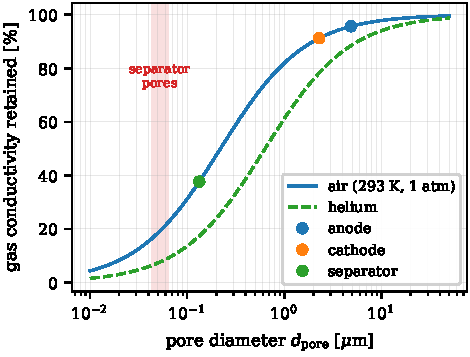
\includegraphics[width=0.55\textwidth]{fig1_knudsen}
\caption{Retained fraction of pore-gas conduction, Eq.~\eqref{eq:knudsen}, at 293\,K and 1\,atm for air (solid) and helium (dashed). Markers: hydraulic pore sizes of the three reference systems (air curve). Shaded band: measured polyolefin-separator pore diameters; inside it, the air mean free path exceeds the pore size.}
\label{fig:knudsen}
\end{figure}

\begin{figure}[tb]\centering
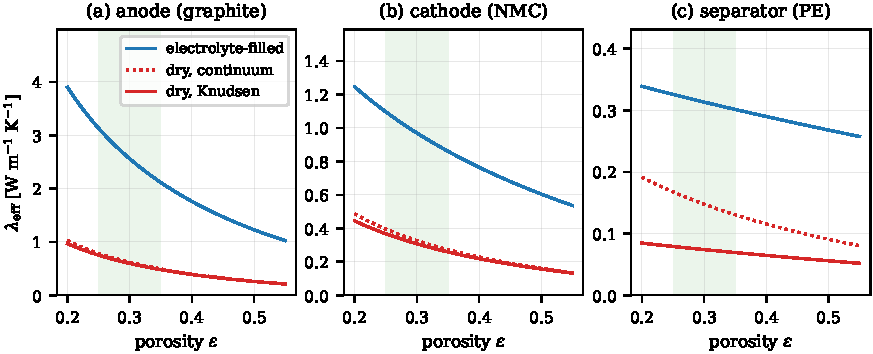
\includegraphics[width=\textwidth]{fig2_maps}
\caption{Zero-fit $\leff(\varepsilon)$ for (a)~graphite anode, (b)~NMC cathode, (c)~PE separator: electrolyte-filled, dry-continuum, and dry-Knudsen variants. Green band: typical post-calendering porosity window.}
\label{fig:maps}
\end{figure}

\subsection{Baseline comparison: morphology is the discriminator}
\label{sec:results:baselines}

Table~\ref{tab:baselines} evaluates the closure hierarchy at the four uncalendered points, the cleanest test because no calender has yet altered any contacts, with identical inputs and Knudsen-corrected helium pore gas throughout. The Wiener bounds are uninformative at graphite's phase contrast, spanning $0.24$ to $32\WmK$. More interesting is that the structure-committed baselines fail in \emph{opposite, morphology-diagnostic} directions. Bruggeman's co-continuous picture effectively hands the solid phase a percolating highway through the medium, so it overshoots wherever the solid is actually granular: $+17\%$ for NMC622 and up to $+465\%$ for graphite. Maxwell--Eucken isolates every particle in a fluid jacket, so heat must repeatedly cross the poorly conducting gas, and it undershoots everywhere ($-11\%$ to $-70\%$). \Mzero{}, spheres touching at points, is the only zero-parameter closure that is both well-ordered across families and accurate where its geometry actually holds: $+2.7\%$ for NMC811, the electrode with the least additive (4\,wt\%) and hard, near-spherical particles. Its systematic \emph{under}-prediction elsewhere ($-29\%$ NMC622, $-36/-39\%$ graphite) is ordered exactly by expected bridge strength (flake-graphite additive in NMC622; soft, plastically self-bridging flakes in the anodes), and along every calendering series the residual walks monotonically from negative to positive: the u-shape is invisible to every porosity-only model, consistent with the documented failure of the two microstructure-resolved models \cite{gandert2023}.

The same diagnostic logic settles the separator. Measured values ($0.07$--$0.18\WmK$) fall between our point-contact lower bound ($0.022$--$0.031$) and a continuous-skeleton parallel-plus-Knudsen upper bound ($0.080$--$0.155$), much closer to the latter, exactly as one expects for a stretched polymer film whose skeleton is co-continuous (Bruggeman, the co-continuous baseline, lands in-range at $0.090$). Here a cautionary observation: a continuum sphere-pack model also reproduces the measured numbers ($0.075$--$0.093$), but it does so the way a broken clock tells the right time twice a day: it overestimates the gas conduction (no Knudsen correction) while underestimating the skeleton connectivity (wrong morphology), and the two errors cancel. The cancellation is fragile, and it breaks the moment the gas or its pressure changes; the two-pressure experiment of Sec.~\ref{sec:experiments} is designed to break it on purpose.

\begin{table}[tb]\centering\footnotesize\setlength{\tabcolsep}{4.5pt}
\caption{Baselines at the uncalendered points (dry, helium pore gas with Knudsen correction, identical constituent inputs; coating values derived from \cite{gandert2023} via Eq.~\eqref{eq:stack}). W$^{-}$/W$^{+}$: Wiener series/parallel bounds; ME: Maxwell--Eucken. All values in $\WmK$.}
\label{tab:baselines}
\begin{tabular}{lcccccc}
\toprule
 & measured & W$^{-}$ & ME & Bruggeman & W$^{+}$ & \Mzero{} (ZBS+Kn)\\
\midrule
graphite (thin), $\varepsilon=0.606$  & 1.429 & 0.242 & 0.430 & 8.07 & 31.6 & \textbf{0.871}\\
graphite (thick), $\varepsilon=0.597$ & 1.405 & 0.245 & 0.441 & 9.07 & 32.3 & \textbf{0.903}\\
NMC622, $\varepsilon=0.513$           & 0.704 & 0.258 & 0.434 & 0.825 & 1.29 & \textbf{0.498}\\
NMC811, $\varepsilon=0.507$           & 0.492 & 0.260 & 0.440 & 0.841 & 1.30 & \textbf{0.505}\\
\bottomrule
\end{tabular}
\end{table}

\begin{figure}[tb]\centering
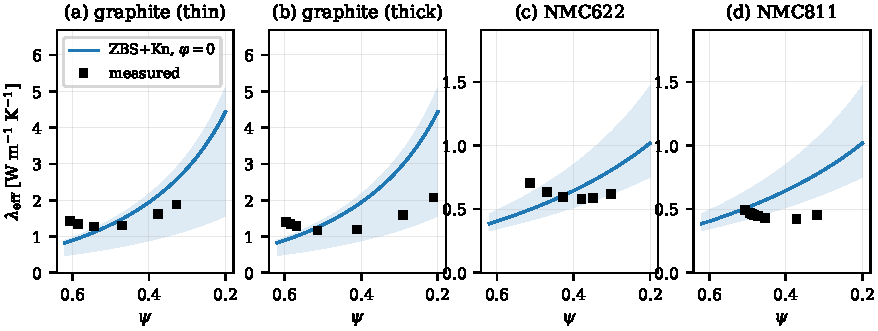
\includegraphics[width=\textwidth]{fig3_zerofit}
\caption{Zero-fit \Mzero{} (dry, helium) against the coating conductivities of all 27 calendering states: (a)~thin and (b)~thick graphite anode, (c)~NMC622, (d)~NMC811. Bands: $\lams$ across the physical anisotropy range. The residuals grow systematically toward low porosity; this is the contact signature.}
\label{fig:zerofit}
\end{figure}

\subsection{Ablation: what each model component buys}
\label{sec:results:ablation}

Table~\ref{tab:ablation} makes each component justify its existence. Adding a \emph{constant} contact fraction (\Mone) more than halves the average error, from $31.1\%$ to $13.5\%$: the as-coated bridge network carries a substantial share of the conduction and cannot be treated as a small correction. Making the contact fraction \emph{process-dependent} (\Mtwo, Eq.~\eqref{eq:phi}) reaches $4.5\%$, the dataset's own scatter of about $5\%$, and reproduces the u-shape (Fig.~\ref{fig:calibrated}): the dip is bridge damage ($a<0$ in all four families) losing against densification, the upturn is densification plus, where it is reached, interlocking recovery. The recovery term $b>0$ appears in exactly the two families where interlocking is independently evidenced: NMC622, whose particles visibly penetrate the soft aluminum foil in electron micrographs at the highest line load \cite{gandert2023}, and the thick anode, which carries the highest line force of the four. The fitted parameters are physically legible across the board: $\varphi_0=0.005$--$0.017$ brackets the VDI rigid-sphere contact fraction of $0.0077$ \cite{vdi}, and the fitted $\lams$ lands in the low, cross-plane-dominated end of graphite's anisotropy band, which is what through-plane transport across lying flakes demands. Held-out transfer completes the picture: within a recipe, the calibration carries over usefully ($20.9\%$ on the thick anode it never saw); across additive recipes it fails ($39.5\%$, NMC622 to NMC811), and the next subsection dissects why.

\begin{table}[tb]\centering\small
\caption{Ablation: MAPE over all calendering states. \Mzero: $\varphi=0$, mid-band $\lams$. \Mone: constant $\varphi$, fitted $(\lams,\varphi_0)$. \Mtwo: full $\varphi(\Pi)$, fitted $(\lams,\varphi_0,a,b)$. Right: \Mtwo{} parameters.}
\label{tab:ablation}
\begin{tabular}{lcccl}
\toprule
Family & \Mzero & \Mone & \Mtwo & \Mtwo{} parameters $(\lams,\varphi_0,a,b)$\\
\midrule
graphite (thin)  & 27.3\% & 9.7\%  & \textbf{1.8\%} & $(24.8,\;0.0094,\;-0.024,\;0)$\\
graphite (thick) & 48.6\% & 17.0\% & \textbf{5.4\%} & $(5.0,\;0.0121,\;-0.042,\;0.053)$\\
NMC622           & 19.1\% & 14.2\% & \textbf{1.4\%} & $(1.6,\;0.0171,\;-0.089,\;0.039)$\\
NMC811           & 29.3\% & 12.9\% & \textbf{9.4\%} & $(1.5,\;0.0048,\;-0.049,\;0)$\\
\midrule
\textbf{average} & \textbf{31.1\%} & \textbf{13.5\%} & \textbf{4.5\%} & \\
\bottomrule
\end{tabular}
\end{table}

\begin{figure}[tb]\centering
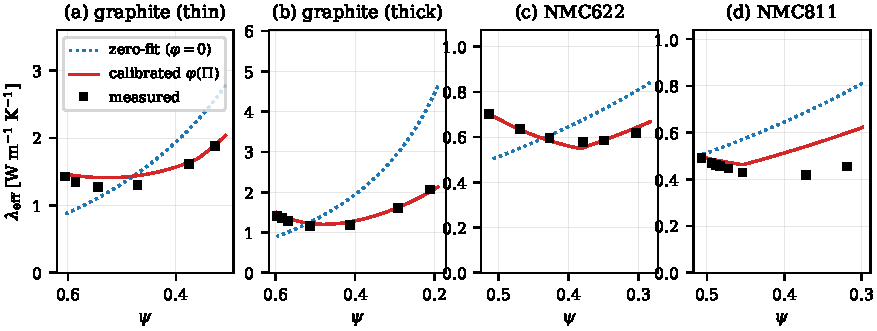
\includegraphics[width=\textwidth]{fig4_calibrated}
\caption{Calibrated \Mtwo{} closure (solid) vs.\ \Mzero{} (dotted) along each family's calendering trajectory; squares: measured coating values. The process-dependent contact term reproduces the u-shape that porosity-only closures cannot.}
\label{fig:calibrated}
\end{figure}

\subsection{Design principles from the fitted parameters}
\label{sec:results:design}

The fitted parameters are measurements of contact physics, and comparing them across recipes yields design rules, provided the comparison is done in the right units. Binder and additive densities ($1.6$--$1.8\,\mathrm{g\,cm^{-3}}$) are far below those of the active materials (NMC: $4.7$), so a recipe quoted in weight percent hides how much \emph{space} the inactive phase occupies; Table~\ref{tab:design} therefore compares in volume. Three interplays emerge. \emph{(i)~Bridge conductance.} The as-coated group $G=\varphi_0\lamb$, normalized per unit inactive volume, is roughly $20\times$ larger for the anodes than for the cathodes: soft graphite flakes deform plastically and bridge each other with high-conductivity contacts all by themselves, whereas hard NMC spheres depend entirely on the additive network between them. Within the cathodes, two weight-percent of flake graphite doubles NMC622's bridge effectiveness over carbon-black-only NMC811: the single clearest recipe lever in the data. \emph{(ii)~Damage rate.} The fractional loss $|a|/\varphi_0$ orders perfectly by binder mechanics: stiff PVDF networks fail $2$--$4\times$ faster per unit compression than elastomeric CMC/SBR, whose rubbery bridges stretch where PVDF's fracture. \emph{(iii)~Recovery} appears only once a process threshold is crossed: NMC811's $b=0$ reflects a calendering window that never reached interlocking ($\Pi\le0.26$), rather than an absence of the underlying mechanism. The design rules: a small flake-graphite additive outperforms additional carbon black by about a factor of two per unit volume; elastomeric co-binders protect the thermal and adhesion network in heavily calendered designs; and the calendering setpoint should not sit in the conductivity/adhesion dip, so either calender lighter or push through into interlocking.

\begin{table}[tb]\centering\small
\caption{Volume-space decomposition of the contact parameters.}
\label{tab:design}
\begin{tabular}{lccccc}
\toprule
Family & binder+additive & $G=\varphi_0\lamb$ & $G/\mathrm{vol}$ & $|a|/\varphi_0$ & binder\\
 & [vol\% of solid] & [$\WmK$] & & [$\Pi^{-1}$] & \\
\midrule
graphite (thin)  & 6.4  & 1.22 & 19.0 & 2.6  & CMC/SBR\\
graphite (thick) & 6.4  & 1.57 & 24.4 & 3.5  & CMC/SBR\\
NMC622           & 17.8 & 0.41 & 2.3  & 5.2  & PVDF\\
NMC811           & 10.0 & 0.12 & 1.2  & 10.2 & PVDF\\
\bottomrule
\end{tabular}
\end{table}

\subsection{Error analysis: identifiability and transfer}
\label{sec:results:errors}

\paragraph{What the data can and cannot determine.}
With four parameters fitted to 6--8 points per family, one must ask which parameters the data actually pin down. Figure~\ref{fig:error}a answers by profile likelihood: fixing $\lams$ anywhere in the range 5--30$\WmK$ and refitting the rest keeps the error within two points of optimal, with $\varphi_0$ compensating between $0.0073$ and $0.0120$; beyond $\lams\approx40$ the fit degrades beyond repair. The data therefore reject the high, in-plane-dominated end of the anisotropy band, consistent with through-plane transport crossing the flakes' weak axis. At the same time, parameter values inside the valley compensate each other, so we report the grouped quantities of Table~\ref{tab:design} together with the valley bounds as the parameter uncertainty, rather than individual point estimates.

\paragraph{Why cross-recipe transfer fails.}
Figure~\ref{fig:error}b dissects the $39.5\%$ transfer failure by hybrid swaps, replacing one parameter group at a time in NMC622's calibration with NMC811's own value. Swapping $\lams$ recovers almost nothing ($36.2\%$). Swapping $\varphi_0$ alone recovers about $90\%$ of the recoverable error ($12.2\%$, against the $9.4\%$ self-fit floor); adding the damage dynamics $(a,b)$ contributes a further $0.3$ points. The conclusion is sharp: cross-recipe failure is recipe physics concentrated in a single parameter, the as-coated bridge conductance set by the conductive-additive system, and not a particle-property or dynamics issue. The practical corollary costs one measurement: re-anchor $\varphi_0$ on one as-coated sheet when changing recipes, and the rest of the calibration travels.

\paragraph{Remaining exposures, quantified.}
The Knudsen jump coefficient $\beta\in[1.5,2.0]$ moves dry electrode predictions by at most $1.7\%$ but the dry separator by $11.7\%$; the proposed two-pressure experiment determines $\beta$ directly for the separator case. Six of 27 sheets lie below the porosity range of the base closure's packed-bed validation, with no visible degradation of the calibrated residuals (the extrapolation is absorbed by $\varphi(\Pi)$, an empirical rather than mechanistic resolution). NMC811's recovery term must not be extrapolated beyond its tested compression range. And all coating values inherit the lumped coating/collector contact resistance of stack metrology \cite{vishwakarma2015}.

\begin{figure}[tb]\centering
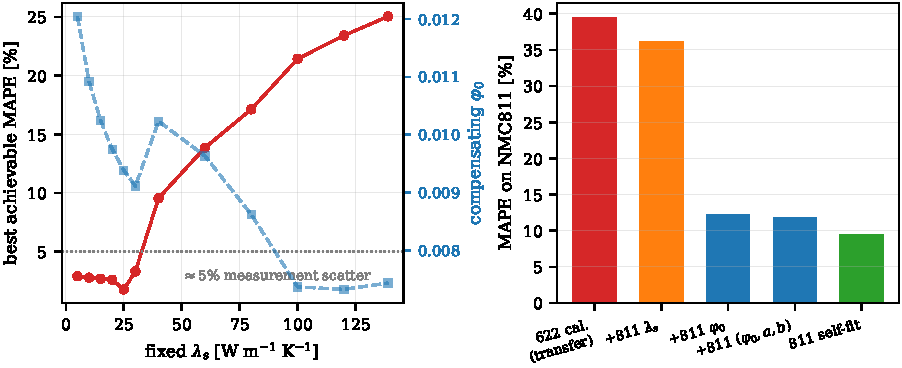
\includegraphics[width=\textwidth]{fig5_error}
\caption{(a)~Profile likelihood over $\lams$ for the thin anode: the $\lams/\varphi_0$ identifiability valley; right axis, the compensating $\varphi_0$. (b)~Hybrid-swap decomposition of the NMC622$\to$NMC811 transfer: the as-coated bridge term $\varphi_0$ carries the failure.}
\label{fig:error}
\end{figure}

\subsection{Bayesian calibration and model evidence}
\label{sec:results:bayes}

Replacing least squares with full posterior sampling (protocol in Sec.~\ref{sec:data:protocol}) answers two questions the point estimates cannot. First, \emph{are the fits trustworthy?} Every posterior median agrees with the corresponding least-squares estimate, the thin-anode $\lams$ posterior spans $7.5$--$30.5\WmK$ at $90\%$ probability, an independent, probabilistic reproduction of the profile-likelihood valley of Sec.~\ref{sec:results:errors}, and the inferred noise levels ($4.7\%$, $8.5\%$, $1.1\%$, $15.6\%$ for the four families) recover each family's actual residual scatter without being told, including NMC811's poorer fit, which the posterior reports honestly as a wider noise level rather than hiding it in overconfident parameters. The $\varphi_0$ credible intervals bracket the VDI rigid-sphere value across families. A pooled fit sharpens the recipe picture: one shared parameter set for both same-recipe graphite electrodes (14 sheets) still describes them to $6.7\%$ and $8.6\%$, so the recipe hypothesis holds to within the thickness-induced interface differences that Sec.~\ref{sec:results:design} identified.

Second, \emph{is the process-dependent contact term statistically necessary, or would a constant contact fraction do?} The widely applicable information criterion (WAIC), which estimates out-of-sample predictive accuracy and penalizes effective model complexity, answers per family (Table~\ref{tab:waic}): the quadratic $\varphi(\Pi)$ is decisively preferred for three of the four families (differences of $13$--$32$, where $\sim$$10$ already counts as strong), with effective parameter counts of $3$--$4$ confirming the model is not overparameterized. The exception is NMC811 ($\Delta=1.6$): for the one family whose calendering window never reached the interlocking regime, the data cannot justify the quadratic over a constant term. The formal model comparison thereby rediscovers, independently, the process-threshold finding of Sec.~\ref{sec:results:design} -- and the evidence for the contact term now rests on three legs: error reduction (Table~\ref{tab:ablation}), mechanism correlation (adhesion), and predictive information criteria.

\begin{table}[tb]\centering\small
\caption{WAIC comparison (lower is better) of constant contact fraction (\Mone) vs.\ the process-dependent quadratic (\Mtwo); $\Delta>0$ favours the quadratic. $p_{\mathrm{WAIC}}$: effective number of parameters of \Mtwo.}
\label{tab:waic}
\begin{tabular}{lcccc}
\toprule
Family & WAIC \Mone & WAIC \Mtwo & $\Delta$ & $p_{\mathrm{WAIC}}$ (\Mtwo)\\
\midrule
graphite (thin)  & $-3.0$ & $-16.0$ & $+13.0$ & 2.9\\
graphite (thick) & $2.2$  & $-10.6$ & $+12.8$ & 2.9\\
NMC622           & $-0.3$ & $-31.8$ & $+31.6$ & 4.2\\
NMC811           & $-0.6$ & $-2.2$  & $+1.6$  & 1.5\\
\bottomrule
\end{tabular}
\end{table}

\subsection{Manufacturing QC applications}
\label{sec:results:qc}

\paragraph{Porosity QC.}
On a synthetic production batch of 200 calendered sheets (true porosities drawn from $\mathcal N(0.30,\,0.012)$, a realistic calender drift, with $3\%$ relative measurement noise), Newton inversion (Eq.~\eqref{eq:newton}) recovers porosity with a root-mean-square error of $0.0078$ absolute and zero bias (Fig.~\ref{fig:qc}). The a-priori prediction of Eq.~\eqref{eq:sigma}, $\sigma_\varepsilon=0.0092$ including the $2\%$ model floor, brackets the observed scatter: the uncertainty model is calibrated and slightly conservative, as is preferable for quality-control use. Against a typical $\pm0.02$ porosity specification this yields $87.5\%$ correct single-shot classification, with all errors confined to genuinely borderline sheets; averaging $n=4$ repeats shrinks the measurement contribution by half and makes the specification window cleanly resolvable.

\paragraph{Interface and delamination QC.}
The calibrated closure decomposes $\leff$ into a core contribution and a bridge contribution, and the split is large: in the as-coated state, which is exactly where post-drying adhesion and binder-migration quality control matters, bridges carry between $16\%$ and $66\%$ of the heat. A failure of the bridge network (delamination, binder maldistribution) therefore shifts a thermal reading by $5$ to $22$ standard deviations of a $3\%$-noise measurement: even partial degradation is detectable in a single shot. The asymmetry with the previous paragraph is worth stating plainly: porosity can already be monitored inline from thickness and mass loading, so thermal porosity QC serves as a convenient secondary check; \emph{interface quality has no inline monitor at all}, and on this evidence a fast thermal reading is its most direct proxy, consistent with the conductivity--adhesion correlation reported independently \cite{gandert2023}.

\begin{figure}[tb]\centering
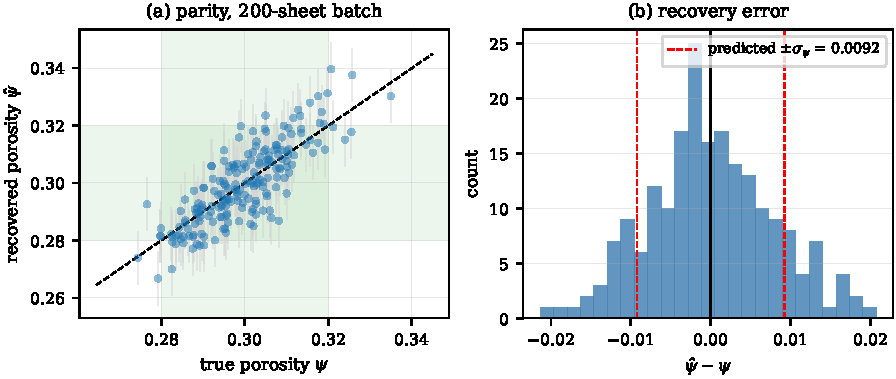
\includegraphics[width=\textwidth]{fig6_qc}
\caption{Inverse porosity QC on a synthetic 200-sheet batch at $3\%$ measurement noise: (a)~parity with predicted $\pm\sigma_\varepsilon$ bars and the $\pm0.02$ specification window; (b)~recovery-error histogram against the first-order uncertainty prediction of Eq.~\eqref{eq:sigma}.}
\label{fig:qc}
\end{figure}

\subsection{From coatings to the cell: an 18650 stack test}
\label{sec:results:stack}

The quantity cell designers actually need is the through-plane conductivity of the full layer stack. Steinhardt et al.\ \cite{steinhardt2021} published both the complete unit-cell structure of a commercial 18650 cell (per-layer thicknesses and porosities; anode $\varepsilon=0.216$, cathode $\varepsilon=0.171$, separator $\varepsilon=0.45$) and its measured jelly-roll conductivity, $k_\perp = 1.122\WmK \pm 6.2\%$, which permits a fully bottom-up test: predict each electrolyte-filled coating with the zero-fit closure at \emph{their} porosities (a genuine extrapolation, far below the calendering window of the calibration data), assemble the repeating unit in series with separator and collector foils, and compare. With perfect interfaces the prediction is $1.29\WmK$, $15\%$ above the measurement -- the physically expected sign and a small magnitude, since the layer-only model neglects all interface resistance. Matching the measurement exactly requires only $\approx6\,\mu\mathrm{K\,m^2\,W^{-1}}$ of contact resistance per coating/separator interface, two orders of magnitude below the $420\,\mu\mathrm{K\,m^2\,W^{-1}}$ measured on an unbonded, torn-down stack \cite{vishwakarma2015}; a jelly roll wound under tension presses its interfaces together, so the implied value is physically coherent. Sweeping the per-interface resistance from torn-down to perfect contact spans predictions from $0.11$ to $1.29\WmK$, which reproduces, almost exactly, the $0.15$--$1.4\WmK$ spread of the entire published cell-level literature \cite{steinhardt2022}: in this reading, much of the literature's apparent disorder is an interface-pressure axis, not disagreement about the coatings. As an independent cross-model anchor, microstructure-resolved simulations \cite{oehlerdiss} place electrolyte-filled anode coatings at $\approx1.9$--$2.3$ and cathode coatings at $\approx0.95$--$1.1\WmK$ at comparable compositions; the closure's values sit at the same level, two unrelated modeling routes agreeing within $10$--$25\%$.

\subsection{Multi-source meta-validation and sensitivity}
\label{sec:results:meta}
Widening the test beyond the calibration source, we predict (zero fit, each material at its literature through-plane particle conductivity) twelve independent coating and separator measurements drawn from three further laboratories and the steady-state method \cite{burheim2013,marconnet2018,richter2017}. The closure tracks them to a median $37\%$ relative error, with $83\%$ of points inside a factor of two, and to within a few percent where the inputs are best characterised (the LCO cathode: $-4\%$ dry, $+5\%$ soaked). The residuals are attributable rather than random: the two independent wet graphite-anode values disagree with \emph{each other} by $\sim50\%$, LMO is the lowest-conductivity cathode oxide and is over-predicted, and the two outlying separator points are a barely-wetted sample and a compacted one. A baseline comparison on the same wet coatings reconciles with the dry-data hierarchy of Table~\ref{tab:baselines}: Bruggeman fails badly (median $185\%$, its co-continuous path percolating the solid), whereas Maxwell--Eucken, which under-predicts at the high contrast of dry coatings, becomes competitive at the low contrast of wet ones ($19\%$) -- but carries no contact or calendering mechanism. The dominant controllable error throughout is the through-plane solid conductivity, the anisotropy point of Sec.~\ref{sec:limitations}. Finally, a converged Sobol decomposition of the dry-anode conductivity ranks porosity first ($S_T=0.46$), the contact pair $(\varphi,\lambda_b)$ a close second ($\approx0.48$ combined), and particle size negligible ($S_T\approx0$, the pore gap being the bottleneck at high contrast) -- a measurement-priority list for process control: fix porosity and the calendering/contact state first.

% =====================================================================
\section{Discussion: choosing among approaches}
\label{sec:discussion}

The results support a clear division of labor between modeling approaches. \emph{Analytic closures} remain the right tool whenever evaluations must be cheap, differentiable, or invertible, which covers cell-level thermal simulation, process optimization, and quality control, but under two conditions that this work makes precise. The geometry must match the material: Sec.~\ref{sec:results:baselines} shows that the baselines' failure pattern is itself the diagnostic, point-contact packing for low-additive electrodes, co-continuity for separators. And the process-dependent contact physics must be represented: by Table~\ref{tab:ablation} it is worth a factor of seven in accuracy, far more than the choice between any two textbook closures. \emph{Microstructure-resolved simulation} is the natural tool for exploring hypothetical microstructures before they exist; its present generators, however, do not encode calender-induced contact evolution \cite{gandert2023}, and embedding a $\varphi(\Pi)$-like contact state into DEM or homogenization generators looks like the obvious synthesis of the two worlds. \emph{Purely data-driven regression} would interpolate the 27 points effortlessly and is the right choice when only interpolation is needed; but it offers no mechanism, no transfer diagnosis when the recipe changes, and no pressure or gas dependence to test. The closure's value lies in the physical interpretability of its parameters, which converts a fitted curve into design rules (Table~\ref{tab:design}), a one-measurement transfer correction (Sec.~\ref{sec:results:errors}), and falsifiable predictions (Sec.~\ref{sec:experiments}). Seen this way, the per-recipe nature of the contact parameters is itself a quantitative result: contact conduction originates in the contact zones, which bulk volume averages cannot resolve, and six calendering states suffice to characterize it for a new recipe.

% =====================================================================
\section{Proposed experimental validation}
\label{sec:experiments}

The model is calibrated on published data; the following campaign (per recipe: about 26 sheets, one calendering afternoon, two measurement days) is designed to test its \emph{mechanisms}, with stated criteria for failure.

\begin{enumerate}
\item \textbf{Sample matrix.} Six calendering states from $\Pi=0$ to the production maximum (single batch, single-side coatings); duplicate as-coated sheets for the $\varphi_0$ re-anchor; each state measured dry and electrolyte-soaked.
\item \textbf{Porosity ground truth.} Areal mass; flat-anvil micrometer thickness at $\le0.3\,\mathrm{N\,mm^{-2}}$ (not a ball-tip dial gauge, which compresses the coating \cite{gandert2023}); helium-pycnometric solid density; GUM uncertainty budget.
\item \textbf{Conductivity.} Through-plane laser flash with penetration-model evaluation \cite{mcmasters}, recording the purge gas (it is the pore gas), or a guarded hot plate; $20\,^\circ$C; $n=4$ repeats per sheet, bringing $3\%$ single-shot noise to $1.5\%$.
\item \textbf{Two-pressure Knudsen discrimination} (decisive for separators; recommended for the most porous electrode state): repeat the dry measurement at about $1000$ and at or below $100$\,mbar chamber pressure. By Eq.~\eqref{eq:knudsen}, pore-gas conduction depends on pressure through $\Kn\propto1/p$, while skeleton and bridge conduction do not. The pressure split therefore isolates the gas channel, pins $\beta$, and deliberately breaks the error cancellation identified for continuum sphere-pack separator models in Sec.~\ref{sec:results:baselines}.
\item \textbf{Adhesion correlation.} Pull-off adhesion strength at every calendering state. Equation~\eqref{eq:phi} claims the conductivity-relevant contact fraction tracks interface damage and interlocking; then $\varphi(\Pi)$ and adhesion must share sign structure and dip location.
\item \textbf{Cross-section image quantification.} Ion-milled SEM cross-sections at each calendering state, with the contact and bridge areas quantified by image segmentation. This yields a direct, microscopy-based estimate of $\varphi(\Pi)$ that is independent of any thermal measurement, and therefore the sharpest available test of the contact interpretation: the image-derived and the thermally fitted contact fractions must agree in magnitude and in the location of the dip.
\item \textbf{Multi-recipe extension and informative design.} Once the first recipe is complete, the same matrix should be repeated across recipes that vary one factor at a time (binder system, conductive-additive type and content, particle size). This builds the data basis for predicting contact parameters from recipe descriptors rather than calibrating each recipe separately. Because the closure is differentiable, the calendering states and chamber pressures of later campaigns need not be evenly spaced: they can be chosen to maximize the expected information gain on the parameters, which concentrates measurements where they discriminate most.
\item \textbf{Acceptance criteria.} (i)~Calibrated residuals at or below the measurement uncertainty at all $\Pi$; (ii)~the pressure split consistent with Eq.~\eqref{eq:knudsen} within the $\beta$ band; (iii)~the $\varphi(\Pi)$--adhesion correlation as predicted; (iv)~the image-derived contact fraction consistent with the thermally fitted one. Failure of (ii) falsifies the Knudsen term as implemented; failure of (iii) or (iv) falsifies the contact interpretation and demotes $\varphi(\Pi)$ to a curve fit.
\end{enumerate}

% =====================================================================
\section{Limitations}
\label{sec:limitations}

(1)~All conclusions about the contact term rest on one (excellent) public dataset: four families, three recipes, one laboratory, one metrology chain; the campaign of Sec.~\ref{sec:experiments} is required before generality can be claimed. (2)~With four parameters on six to eight points per family, $\lams$ and $\varphi_0$ are partially confounded at $\Pi=0$; we therefore report the profile-likelihood valley and grouped quantities rather than over-interpreting point estimates. (3)~The quadratic $\varphi(\Pi)$ is phenomenology anchored to adhesion observations, not derived contact mechanics, and $b$ is unconstrained outside each family's tested compression range. (4)~Stack-derived coating values lump the coating/collector contact resistance; free-standing-film metrology would separate it. (5)~Electrode porosities extrapolate the porosity range of the base closure's packed-bed validation; the extrapolation is handled empirically, not mechanistically. (6)~The sphere-pack geometry is wrong for stretched-film separators, so we claim only bounds there, never point predictions. (7)~Anisotropy is compressed into one scalar effective $\lams$; in-plane conduction and genuinely anisotropic unit cells are out of scope. (8)~Wet-state predictions assume fully saturated pores; partial wetting during electrolyte filling is untreated. (9)~\emph{Measurement-method dependence of the absolute scale.} The calibration data were acquired by laser-flash analysis (LFA); a recent methodological study \cite{gandert2025} reports that LFA and the guarded-hot-plate (GHP) method disagree systematically, with flash diffusivity -- which excludes inter-sample contact resistance -- yielding cross-plane conductivities up to roughly twice the steady-state GHP values. This sets a ceiling on the transferable accuracy of the \emph{absolute} fitted parameters ($\lams$, and through the confound $\varphi_0$): a model calibrated on LFA data predicts LFA-scale conductivities. Two mitigating facts keep the central claims intact. First, the effect is close to a multiplicative scale factor, so the \emph{shape} of $\varphi(\Pi)$, the u-shape, the ablation hierarchy, the WAIC model selection, and the recipe-transfer decomposition -- all of which are relative or structural -- are method-robust. Second, the very interfacial resistance that GHP includes and LFA omits is precisely the contact physics our 18650 stack test (Sec.~\ref{sec:results:stack}) treats explicitly, so the two methods bracket the application: LFA for the bare coating property, GHP for the as-installed stack. A clean resolution is the same campaign already specified -- measuring one recipe by both methods alongside the two-pressure protocol pins the scale factor directly.

% =====================================================================
\section{Conclusion}
\label{sec:conclusion}

A minimal, physically interpretable extension of the ZBS closure, Knudsen-corrected pore gas plus a compression-indexed contact term, closes the gap between packed-bed theory and calendered battery electrodes. It quantifies a rarefaction correction that had previously been noted but not evaluated; it outperforms the classical effective-medium hierarchy with zero fitted parameters; calibrated, it reaches the measurement noise floor ($4.5\%$ over 27 calendering states) and reproduces the measured u-shaped conductivity--calendering dependence that defeated previous models; Bayesian posteriors and information criteria corroborate both the calibration and the necessity of the process-dependent term; and a bottom-up prediction of a measured commercial 18650 cell within $+15\%$ closes the chain from packed-bed theory to the cell-level quantity that motivated the work. Its fitted parameters function as measurements of contact physics: they decompose into design rules for additive choice, binder mechanics, and calendering setpoint; their identifiability is honestly bounded by profile likelihood; and their transfer behavior localizes all recipe dependence in a single re-anchorable number. Differentiability turns the same closure into manufacturing instrumentation, recovering porosity to $\pm0.008$ from one thermal reading and offering the first candidate inline monitor for interface quality. The specified two-pressure campaign will test this mechanism. Beyond it, several directions remain open. On the experimental side: measurements across additional recipes and coating processes to probe the generality of the contact decomposition, and microscopy-based quantification of the bridge network as an independent observable for $\varphi(\Pi)$. On the modelling side: an anisotropic unit cell for in-plane conduction, partial-saturation states during electrolyte filling, and the embedding of a $\varphi(\Pi)$-like contact state into microstructure-resolved structure generators. On the statistical side, two extensions are prepared in the accompanying repository: learning the mapping from recipe descriptors to contact parameters once several recipes have been measured, with measurement matrices designed for maximum information gain; and electrode-specific conformal calibration of the model uncertainty. On the application side: the integration of the inverse closure into inline calendering and drying quality control, including residual-based anomaly monitoring, and field-type inverse problems such as spatially resolved interface quality reconstructed from flash-thermography image sequences, which is the natural entry point for physics-informed neural networks; for the scalar parameter recovery treated here they offer no advantage over classical optimization.

% =====================================================================
\section*{Reproducibility statement}
The complete project, the JAX implementation of the closure (with a regression test enforcing the exact $\varphi=0$ reduction to the validated base model), the transcribed datasets with row-level source citations, all calibration scripts with the objective, bounds, and seeds stated in Sec.~\ref{sec:data:protocol}, the executed analysis notebooks, a 14-test suite that locks every headline number of this paper against silent drift, and the pipeline that regenerates every figure from raw inputs with no hard-coded values, is openly available at:
\begin{center}
\url{https://github.com/j-stoerk/zehner-electrode-thermal}
\end{center}

\section*{Data availability}
The transcribed datasets in \texttt{data/raw/} of the repository above (the calendering transcription and the separator/electrode literature anchors) carry per-row citations to the primary sources \cite{gandert2023,richter2017,marconnet2018,burheim2013,vishwakarma2015}; the primary calendering dataset is published open access by its authors.

\section*{Acknowledgments}
The author thanks Sebastian Schebesta (VARTA Microbattery) for his support of this work, Jochen Eser for mentorship and for first pointing toward Zehner's work, and Prof.\ Carsten Schilde (Technische Universit\"at Braunschweig) for doctoral supervision. This work was supported by the German Federal Ministry of Education and Research (BMBF) within the project GranuGoIn (grant no.\ 03XP0635A), administered by Projekttr\"ager J\"ulich (PTJ).

% =====================================================================
\begin{thebibliography}{99}\small

\bibitem{bandhauer2011}
T.~M. Bandhauer, S.~Garimella, T.~F. Fuller,
A critical review of thermal issues in lithium-ion batteries,
\emph{J. Electrochem. Soc.} \textbf{158} (2011) R1--R25.

\bibitem{richter2017}
F.~Richter, S.~Kjelstrup, P.~J.~S. Vie, O.~S. Burheim,
Thermal conductivity and internal temperature profiles of Li-ion secondary batteries,
\emph{J. Power Sources} \textbf{359} (2017) 592--600.

\bibitem{steinhardt2021}
M.~Steinhardt et al.,
Low-effort determination of heat capacity and thermal conductivity for cylindrical 18650 and 21700 lithium-ion cells,
\emph{J. Energy Storage} \textbf{42} (2021) 103065.

\bibitem{oehlerdiss}
D.~Oehler,
\emph{Bestimmung der thermischen Transporteigenschaften por\"oser Elektroden von Lithium-Ionen Batterien},
Dissertation, KIT Scientific Publishing, Karlsruhe, 2021. DOI 10.5445/KSP/1000136047.

\bibitem{steinhardt2022}
M.~Steinhardt, J.~V. Barreras, H.~Ruan, B.~Wu, G.~J. Offer, A.~Jossen,
Meta-analysis of experimental results for heat capacity and thermal conductivity in lithium-ion batteries: A critical review,
\emph{J. Power Sources} \textbf{522} (2022) 230829.

\bibitem{gandert2023}
J.~C. Gandert, M.~M\"uller, S.~Paarmann, O.~Queisser, T.~Wetzel,
Effective thermal conductivity of lithium-ion battery electrodes in dependence on the degree of calendering,
\emph{Energy Technol.} \textbf{11} (2023) 2300259.

\bibitem{gandert2025}
J.~C. Gandert et al.,
Challenges of the measurement of the effective thermal conductivity of battery electrodes with laser flash analysis and guarded hot plate method,
\emph{Energy Technol.} (2025) 2501125. [Verify volume/pages before submission.]

\bibitem{oehler2021}
D.~Oehler, P.~Seegert, T.~Wetzel,
Modeling the thermal conductivity of porous electrodes of Li-ion batteries as a function of microstructure parameters,
\emph{Energy Technol.} \textbf{9} (2021) 2000574.

\bibitem{sangros2017}
C.~Sangr\'os Gim\'enez, B.~Finke, C.~Schilde, L.~Frob\"ose, A.~Kwade,
Numerical simulation of the behavior of lithium-ion battery electrodes during the calendaring process via the discrete element method,
\emph{Powder Technol.} \textbf{349} (2019) 1--11.

\bibitem{vishwakarma2015}
V.~Vishwakarma, C.~Waghela, Z.~Wei, R.~Prasher, S.~C. Nagpure, J.~Li, F.~Liu, C.~Daniel, A.~Jain,
Heat transfer enhancement in a lithium-ion cell through improved material-level thermal transport,
\emph{J. Power Sources} \textbf{300} (2015) 123--131.

\bibitem{zehner1970}
P.~Zehner, E.~U. Schl\"under,
W\"armeleitf\"ahigkeit von Sch\"uttungen bei m\"a\ss{}igen Temperaturen,
\emph{Chem. Ing. Tech.} \textbf{42} (1970) 933--941.

\bibitem{bauer1978}
R.~Bauer, E.~U. Schl\"under,
Effective radial thermal conductivity of packings in gas flow. Part II,
\emph{Int. Chem. Eng.} \textbf{18} (1978) 189--204.

\bibitem{vdi}
E.~Tsotsas,
Thermal conductivity of packed beds,
in: \emph{VDI Heat Atlas}, 2nd ed., Ch.~D6.3, Springer, Berlin, 2010.

\bibitem{wiener1912}
O.~Wiener,
Die Theorie des Mischk\"orpers f\"ur das Feld der station\"aren Str\"omung,
\emph{Abh. Math.-Phys. Kl. K\"onigl. S\"achs. Ges. Wiss.} \textbf{32} (1912) 509--604.

\bibitem{hashin1962}
Z.~Hashin, S.~Shtrikman,
A variational approach to the theory of the effective magnetic permeability of multiphase materials,
\emph{J. Appl. Phys.} \textbf{33} (1962) 3125--3131.

\bibitem{maxwell1891}
J.~C. Maxwell,
\emph{A Treatise on Electricity and Magnetism}, 3rd ed., Vol.~1,
Clarendon Press, Oxford, 1891.

\bibitem{eucken1932}
A.~Eucken,
Die W\"armeleitf\"ahigkeit keramischer feuerfester Stoffe: ihre Berechnung aus der W\"armeleitf\"ahigkeit der Bestandteile,
\emph{VDI-Forschungsheft} \textbf{353}, VDI-Verlag, Berlin, 1932.

\bibitem{bruggeman1935}
D.~A.~G. Bruggeman,
Berechnung verschiedener physikalischer Konstanten von heterogenen Substanzen. I,
\emph{Ann. Phys.} \textbf{416} (1935) 636--664.

\bibitem{kennard1938}
E.~H. Kennard,
\emph{Kinetic Theory of Gases},
McGraw-Hill, New York, 1938.

\bibitem{kaganer1969}
M.~G. Kaganer,
\emph{Thermal Insulation in Cryogenic Engineering},
Israel Program for Scientific Translations, Jerusalem, 1969.

\bibitem{burheim2013}
O.~S. Burheim, M.~A. Onsrud, J.~G. Pharoah, F.~Vullum-Bruer, P.~J.~S. Vie,
Thermal conductivity, heat sources and temperature profiles of Li-ion secondary batteries,
\emph{ECS Trans.} \textbf{58} (2014) 145--171 (224th ECS Meeting, Abs.~1190).

\bibitem{marconnet2018}
Y.~Sun, R.~Kantharaj, A.~Marconnet,
Characterization of thermal conductivity and thermal transport in lithium-ion batteries,
Thermal \& Fluids Analysis Workshop (TFAWS), NASA JSC, Houston, TX, 2018.

\bibitem{maleki1999}
H.~Maleki, S.~Al~Hallaj, J.~R. Selman, R.~B. Dinwiddie, H.~Wang,
Thermal properties of lithium-ion battery and components,
\emph{J. Electrochem. Soc.} \textbf{146} (1999) 947--954.

\bibitem{mcmasters}
R.~L. McMasters, J.~V. Beck, R.~B. Dinwiddie, H.~Wang,
Accounting for penetration of laser heating in flash thermal diffusivity experiments,
\emph{J. Heat Transfer} \textbf{121} (1999) 15--21.

\end{thebibliography}

\end{document}
